\documentclass[landscape,xcolor={table},10pt]{beamer}

\usepackage{amsmath}
\usepackage{graphicx}
\usepackage[english]{babel}
\usetheme{Antibes}
\usepackage{tikz}
\usepackage{multimedia}
\usepackage{textpos}
\usepackage{hyperref}
\usepackage{url}
\usepackage{siunitx}

\usetheme{default}
\usecolortheme{seahorse}
\usefonttheme[onlymath]{serif}
\setbeamertemplate{caption}[numbered]
\graphicspath{ {images/} }

\setbeamertemplate{title page}{

        \begin{picture}(0,0)

            

            \put(-168,-100){%
                \begin{minipage}[b][45mm][t]{226mm}
                
                	\centering
               
                  {\usebeamerfont{title}\color{black}\inserttitle \par}
                  
                  \color{black}\insertauthor
                  
                  \insertinstitute
                  
                  \insertdate
                  
                
                  
                \end{minipage}
            }

            \end{picture}
            
           

    }

\title[...]{
\includegraphics[width=2cm]{images/moses_logo_with_text}  \\Analysing the Spectral Content of MOSES Images \\Using Cross Correlation}
\author[Parker]{Jake Parker}
\institute{}
\date{July 22nd, 2015 \\ }

\addtobeamertemplate{frametitle}{}{%
\begin{textblock*}{100mm}(.45\textwidth,-1.7cm)

\end{textblock*}}

	
\begin{document}

	\begin{frame}[plain]
	        \titlepage
	\end{frame}
	\begin{frame}
		\frametitle{Subtracted MOSES Images}
{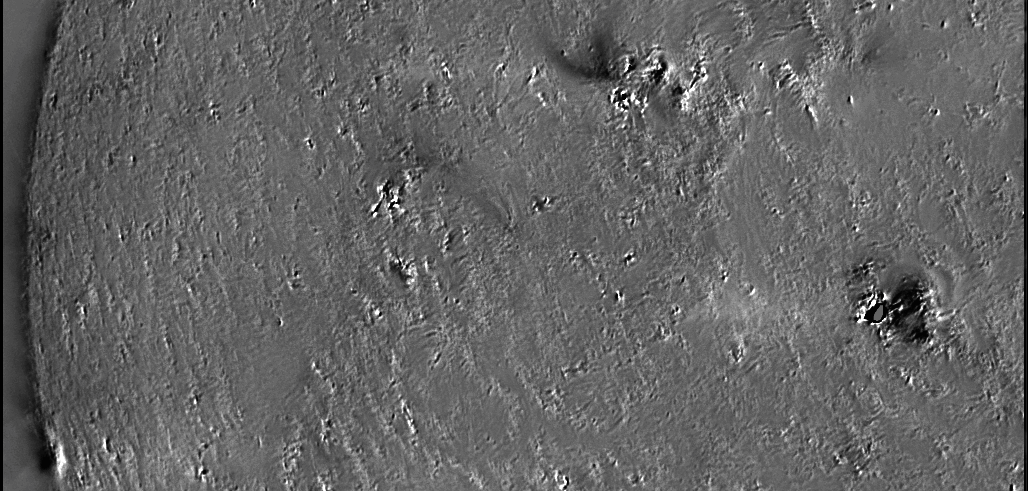
\includegraphics[scale=.3]{images/plus-zero_3.png}	}	
		
	\end{frame}
	\begin{frame}
		
		\frametitle{Cross Correlation}
\\Continuous Definition			
			\begin{itemize}
				\item $ (f \otimes g) (z) \equiv \int_{-\infty}^{\infty} f^*(x) g(x+z) dx$
				\item $(f \otimes g) (z) \equiv \mathcal{F}^{-1} \lbrace \tilde{f}^* (k) \tilde{g}(k)\rbrace$
			\end{itemize}
			
\\Finite Definition
	
$$ (x \otimes y) (z) \equiv \dfrac{ \sum_{n=0}^{N-z-1} (x_n-\bar{x}_n)(y_{n+z}-\bar{y}_{n+z})   }{\sqrt{[\sum_{n=0}^{N-1-L} (x_n-\bar{x}_n)^2][\sum_{n=0}^{N-z-1} (y_{n+z}-\bar{y}_{n+z})^2 ]}}$$
	
			
	

\end{frame}
	\begin{frame}
		\frametitle{Correlation Functions}
		
		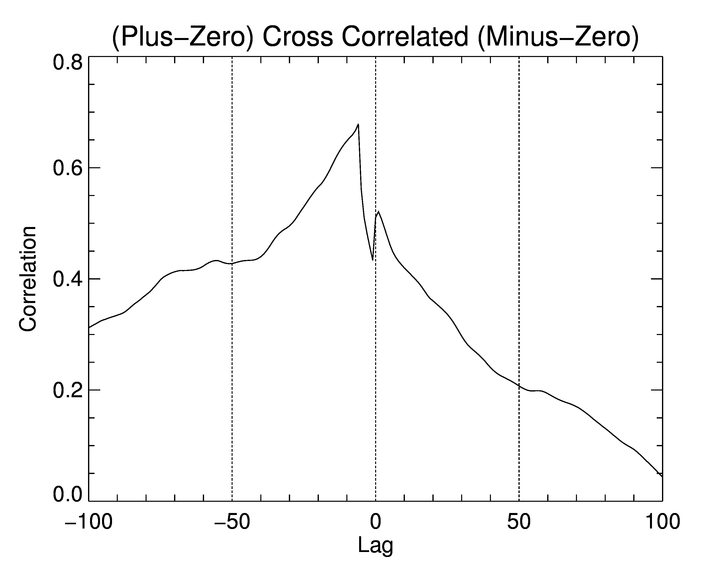
\includegraphics[scale=.23,top]{images/PZ_cc_MZ_3.png}
		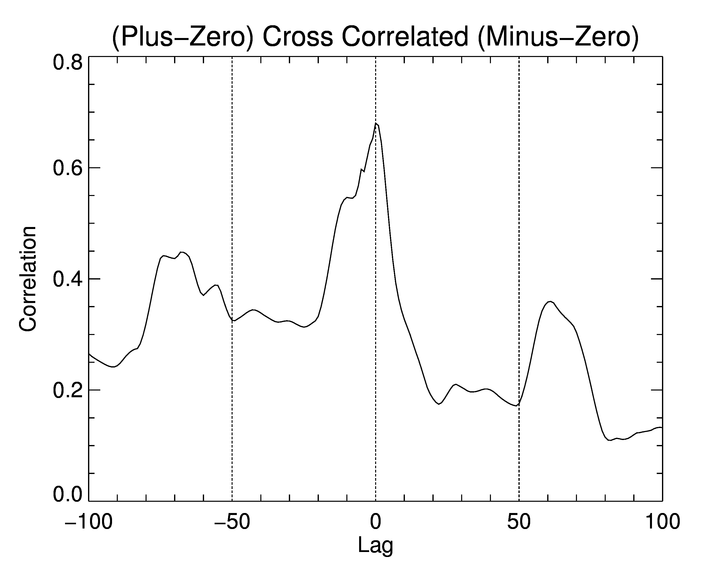
\includegraphics[scale=.23,bottom]{images/pz_cc_mz_3_wishbone.png}
	\end{frame}
	
	\begin{frame}
		\frametitle{Correlation for Large Lag}
	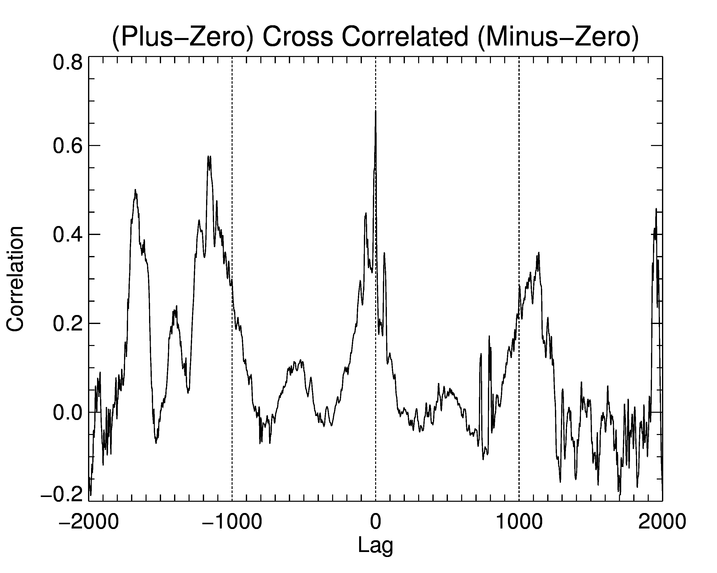
\includegraphics[scale=.37]{images/wishbone_long.png}
	\end{frame}
	
\begin{frame}
	\frametitle{MOSES Throughput}
	
	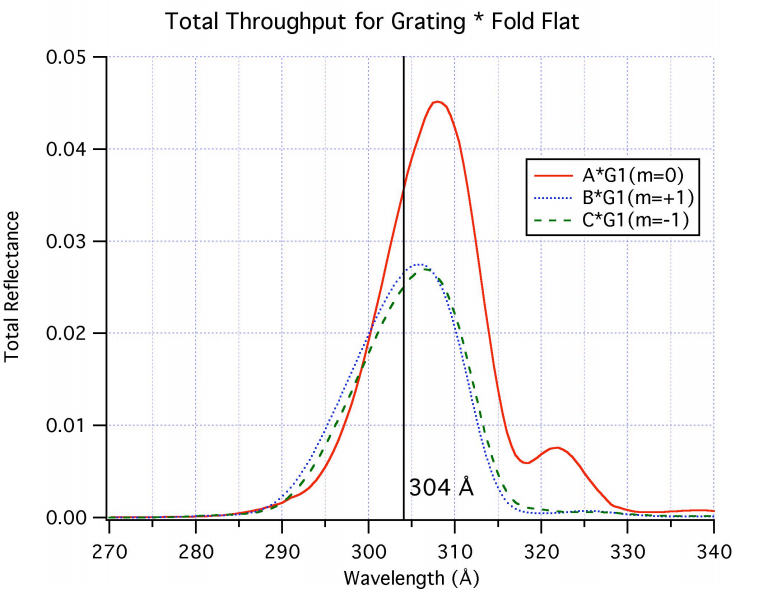
\includegraphics[scale=.35]{images/MOSES_throughput.png}
\end{frame}	
	
\end{document}








